\documentclass[10.5pt,a4paper]{article}
\usepackage[a4paper,margin=2.2cm,top=2.3cm,bottom=2.4cm]{geometry}
\usepackage{fontspec}
\usepackage{unicode-math}
\setmainfont{TeX Gyre Pagella}
\setsansfont{Inter}[Scale=0.88]
\setmonofont{DejaVu Sans Mono}[Scale=0.80]
\setmathfont{DejaVu Math TeX Gyre}[Scale=0.95]
\usepackage{microtype}
\usepackage{xcolor}
\definecolor{accent}{HTML}{1F4E79}
\definecolor{muted}{HTML}{5F6670}
\definecolor{codebg}{HTML}{F6F7F9}
\definecolor{rule}{HTML}{D9DCE1}
\usepackage{graphicx}
\usepackage{booktabs,tabularx,array}
\usepackage{enumitem}
\setlist{nosep,leftmargin=1.4em,topsep=3pt}
\usepackage[font=small,labelfont={bf,sf},labelsep=period,skip=4pt]{caption}
\usepackage{titlesec}
\titleformat{\section}{\sffamily\large\bfseries\color{accent}}{\thesection}{0.7em}{}
\titleformat{\subsection}{\sffamily\normalsize\bfseries}{\thesubsection}{0.6em}{}
\titleformat{\subsubsection}[runin]{\sffamily\small\bfseries}{}{0em}{}[.]
\titlespacing*{\section}{0pt}{14pt}{6pt}
\titlespacing*{\subsection}{0pt}{10pt}{4pt}
\usepackage{fancyhdr}
\pagestyle{fancy}\fancyhf{}
\renewcommand{\headrulewidth}{0.4pt}
\renewcommand{\headrule}{\hbox to\headwidth{\color{rule}\leaders\hrule height \headrulewidth\hfill}}
\fancyhead[L]{\sffamily\footnotesize\color{muted}\ReportShortTitle}
\fancyhead[R]{\sffamily\footnotesize\color{muted}S. K. Eshraghi Naeini}
\fancyfoot[C]{\sffamily\footnotesize\color{muted}\thepage}
\usepackage{listings}
\lstdefinelanguage{VerilogX}[]{Verilog}{morekeywords={localparam,integer,genvar,generate,endgenerate}}
\lstset{language=VerilogX,basicstyle=\ttfamily\footnotesize,keywordstyle=\color{accent}\bfseries,
  commentstyle=\color{muted}\itshape,stringstyle=\color{teal!70!black},numbers=left,numberstyle=\tiny\color{muted},
  numbersep=6pt,backgroundcolor=\color{codebg},frame=single,rulecolor=\color{rule},framesep=4pt,
  xleftmargin=14pt,breaklines=true,columns=fullflexible,keepspaces=true,showstringspaces=false,
  tabsize=4,aboveskip=6pt,belowskip=6pt}
\usepackage{tikz}
\usetikzlibrary{arrows.meta,positioning,shapes.geometric,calc,fit,automata}
\tikzset{blk/.style={draw=accent,thick,fill=accent!6,rounded corners=2pt,minimum height=8mm,minimum width=20mm,align=center,font=\sffamily\small},
         io/.style={font=\sffamily\footnotesize,align=center},
         arr/.style={-{Stealth[length=2mm]},semithick},
         st/.style={state,draw=accent,thick,fill=accent!6,minimum size=9mm,font=\sffamily\footnotesize,inner sep=1pt,align=center}}
\usepackage{xurl}
\usepackage[colorlinks=true,linkcolor=accent,urlcolor=accent,citecolor=accent]{hyperref}
\usepackage{siunitx}
\sisetup{group-separator={,},group-minimum-digits=4}
\newcommand{\sig}[1]{\texttt{#1}}
\newcommand{\pass}{\textcolor{green!45!black}{\textsf{\textbf{PASS}}}}
\newcommand{\repo}{https://github.com/seyedkiarash/seyedkiarash.github.io/tree/main/labs/logic-circuits-lab}
\newcommand{\note}[1]{\par\smallskip\noindent\colorbox{accent!7}{\parbox{\dimexpr\linewidth-2\fboxsep}{\small #1}}\par\smallskip}
\setlength{\parindent}{0pt}
\setlength{\parskip}{4pt}

\newcommand{\ReportTitle}[3]{%
  \thispagestyle{plain}
  {\sffamily\small\color{muted}Logic Circuits Laboratory \textbullet\ Department of Electrical Engineering, Sharif University of Technology\par}
  \vspace{2pt}
  {\sffamily\LARGE\bfseries #1\par}
  \vspace{1pt}
  {\sffamily\Large #2\par}
  \vspace{6pt}
  {\color{rule}\hrule height 0.6pt}
  \vspace{5pt}
  {\small
  \begin{tabular}{@{}l@{\hspace{2em}}l@{}}
    \textcolor{muted}{Student}  & Seyed Kiarash Eshraghi Naeini (403101383)\\
    \textcolor{muted}{Instructor} & Dr.\ Mohammad Reza Movahhedin \quad\textcolor{muted}{Teaching assistant:} Hossein Moghim\\
    \textcolor{muted}{Semester} & Fall 2025 \quad\textcolor{muted}{session:} #3\\
    \textcolor{muted}{Platform} & Zynq-7010 (XC7Z010-CLG400-1), \SI{50}{MHz} clock, Vivado 2019.1
  \end{tabular}\par}
  \vspace{4pt}
  {\color{rule}\hrule height 0.6pt}
  \vspace{8pt}}

\newcommand{\ReportShortTitle}{Experiment 6 -- Sequential logic, clocking and the Zynq PS}
\begin{document}
\ReportTitle{6}{Sequential Logic: Clock Division, LED Patterns, Games and Zynq PS Clocking}{21--22 December 2025}

\section*{Summary}
This experiment moves from combinational to clocked designs. It starts by observing the
\SI{50}{MHz} clock directly, builds a counter-based divider to blink an LED, and uses it for an LED
``flow'' pattern whose speed is adjusted with push buttons. Two block-design projects follow: a reaction
game whose difficulty sets the frequency of its own clock, and the same LED pattern clocked by the ARM
processing system (PS) of the Zynq instead of a board oscillator. Two versions of a ping-pong game
complete the experiment; the second replaces the divided clock by clock-enable pulses in a single clock
domain. All designs were re-verified with self-checking testbenches (7/7 pass); the Vivado reports of
the lab session show all timing met. Code: \url{\repo/lab06-sequential-zynq}.

\section{Part 1 -- Seeing the clock}
\subsection{1a -- Clock on an LED}
Connecting the clock to an LED (\sig{assign LED[0] = clk}) gives an LED that looks steadily lit at roughly
half brightness: it switches \num{50} million times per second, far beyond what the eye can follow.
Vivado warns that a clock net drives an output, which is expected here.

\subsection{1b -- Blinking LED}
A 32-bit counter toggles the LED every \num{80000000} cycles, i.e.\ every \SI{1.6}{s}
(period \SI{3.2}{s}). The testbench (half-period shortened to 10 cycles) checks 25 toggles, each exactly
one half-period apart.

\section{Part 2 -- LED flow with adjustable speed}
A 10-state counter drives the five board LEDs with a fill-then-empty pattern (Fig.~\ref{fig:flow}).
A timer advances the state every $\text{max\_count}+1$ cycles -- initially \num{25000001} cycles,
about \SI{0.5}{s}. The value of \sig{max\_count} is a register: a rising edge on \sig{button[1]} shifts it
left (step time $\times2$) and on \sig{button[2]} shifts it right (step time $/2$). Edges are detected by
comparing each button with its value one clock earlier, so holding a button changes the speed only once.

\begin{figure}[h]
\centering
\begin{minipage}{0.3\linewidth}\centering
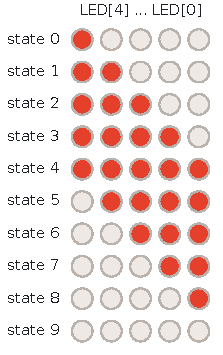
\includegraphics[width=\linewidth]{figures/lab06_ledflow.pdf}
\end{minipage}\hfill
\begin{minipage}{0.64\linewidth}
\begin{lstlisting}
always @(posedge clk) begin           // speed control
    last_b1 <= button[1];
    last_b2 <= button[2];
    if (button[1] & ~last_b1)
        max_count <= max_count << 1;  // slower
    else if (button[2] & ~last_b2)
        max_count <= max_count >> 1;  // faster
end
always @(posedge clk)                 // step timer
    if (t >= max_count) begin
        t     <= 0;
        state <= (state == 9) ? 0 : state + 1;
    end else
        t <= t + 1;
\end{lstlisting}
\end{minipage}
\caption{Part 2: the ten LED states and the speed-control / timer logic.}\label{fig:flow}
\end{figure}

Simulation (initial \sig{max\_count} = 7): the pattern is correct for 20 consecutive steps; a step lasts
8 cycles, 15 after \sig{button[1]} and 4 after two presses of \sig{button[2]}.

\section{Part 3 -- Reaction game (block design)}
\subsection{Design}
A light runs across the five LEDs. The player must press \sig{button[2]} while the \emph{middle} LED is
lit. A hit raises the level and restarts the run faster; a hit on level 3 wins (all LEDs on); a press on
any other LED drops back to level 0. The game was assembled in Vivado IP Integrator from two RTL
modules (Fig.~\ref{fig:game}): the game FSM drives its \sig{mode} (level) output back into the divider that
generates its own clock, giving 4, 6, 8 and \SI{10}{Hz} for levels 0--3.

\begin{figure}[h]
\centering
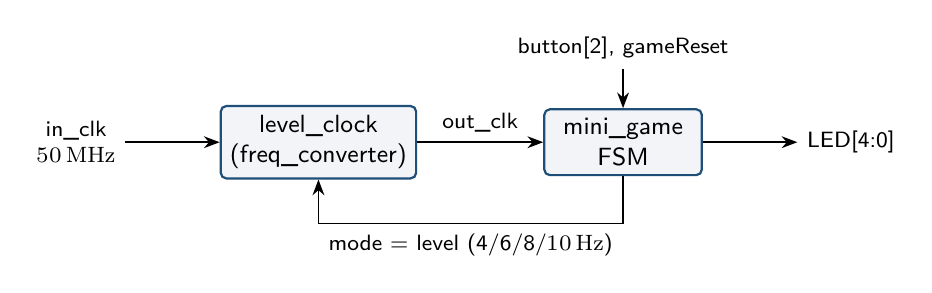
\begin{tikzpicture}[node distance=7mm and 12mm]
  \node[io] (clk) {in\_clk\\\SI{50}{MHz}};
  \node[blk,right=of clk] (div) {level\_clock\\(freq\_converter)};
  \node[blk,right=16mm of div] (game) {mini\_game\\FSM};
  \node[io,right=of game] (led) {LED[4:0]};
  \node[io,above=5mm of game] (btn) {button[2], gameReset};
  \draw[arr] (clk) -- (div);
  \draw[arr] (div) -- node[above,io]{out\_clk} (game);
  \draw[arr] (game) -- (led);
  \draw[arr] (btn) -- (game);
  \draw[arr] (game.south) -- ++(0,-6mm) -| node[pos=0.25,below,io]{mode = level (4/6/8/\SI{10}{Hz})} (div.south);
\end{tikzpicture}\\[6pt]
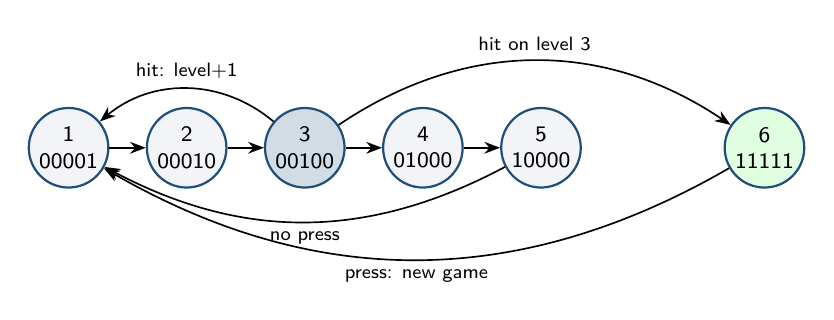
\begin{tikzpicture}[->,>={Stealth[length=2mm]},node distance=15mm,semithick,font=\sffamily\scriptsize]
  \node[st] (s1) {1\\00001};
  \node[st,right of=s1] (s2) {2\\00010};
  \node[st,right of=s2,fill=accent!20] (s3) {3\\00100};
  \node[st,right of=s3] (s4) {4\\01000};
  \node[st,right of=s4] (s5) {5\\10000};
  \node[st,right=18mm of s5,fill=green!12] (s6) {6\\11111};
  \path (s1) edge (s2) (s2) edge (s3) (s3) edge (s4) (s4) edge (s5)
        (s5) edge[bend left=28] node[below]{no press} (s1)
        (s3) edge[bend right=40] node[above]{hit: level+1} (s1)
        (s3) edge[bend left=34] node[above]{hit on level 3} (s6)
        (s6) edge[bend left=30] node[below]{press: new game} (s1);
\end{tikzpicture}
\caption{Part 3: block design (top) and game FSM (bottom). A press in states 1, 2, 4 or 5 is a miss
(level 0, back to state 1).}\label{fig:game}
\end{figure}

\subsection{Verification}
The FSM was unit-tested with a testbench-driven game clock: four hits on the middle LED reach the win
state, and after a new game, a hit followed by a miss returns the level to 0 (Fig.~\ref{fig:gamewave}).
\begin{figure}[h]
\centering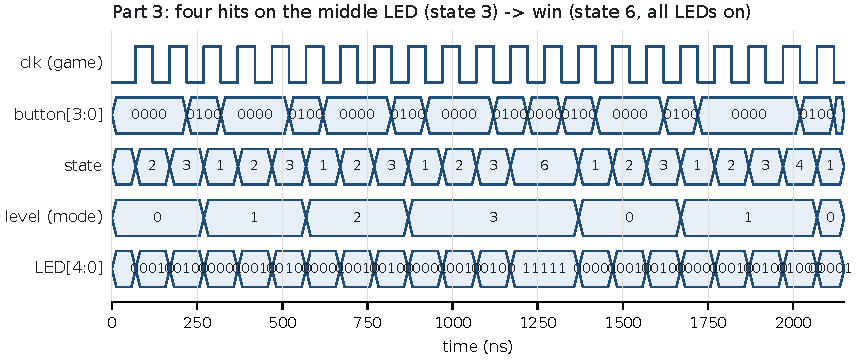
\includegraphics[width=0.92\linewidth]{figures/lab06_minigame_wave.pdf}
\caption{Part 3 simulation: \sig{button[2]} pressed whenever the middle LED (\texttt{00100}) is lit.}\label{fig:gamewave}
\end{figure}

\section{Part 4 -- Clocking the logic from the Zynq PS}
The Zynq-7000 combines an ARM processing system (PS) with the FPGA fabric (PL). In this part the
\sig{processing\_system7} IP is configured to output \sig{FCLK\_CLK0} = \SI{50}{MHz}, and the LED-flow module
of Part 2 is added to the block design as a module reference clocked by it (Fig.~\ref{fig:zynq}). The
constraint file therefore contains only the button and LED pins -- no clock pin -- and Vivado derives the
clock constraint (\sig{clk\_fpga\_0}, \SI{20}{ns}) from the PS configuration. The PS must be configured
(through the boot image or the debugger) before the PL clock runs.

\begin{figure}[h]
\centering
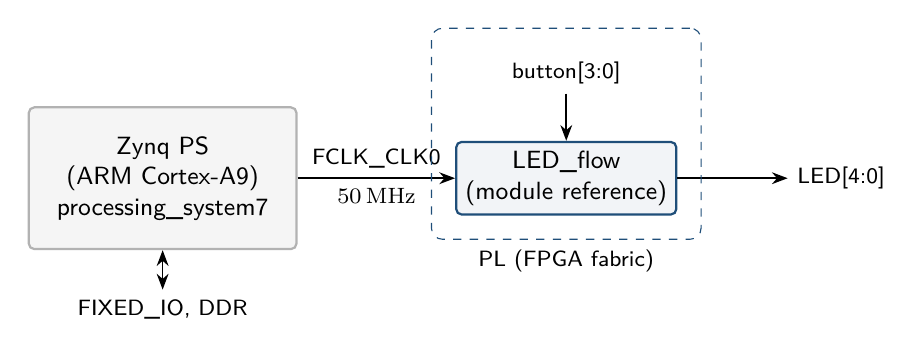
\begin{tikzpicture}[node distance=6mm and 14mm]
  \node[blk,minimum width=34mm,minimum height=18mm,fill=gray!8,draw=gray!60] (ps) {Zynq PS\\(ARM Cortex-A9)\\processing\_system7};
  \node[blk,right=20mm of ps] (lf) {LED\_flow\\(module reference)};
  \node[io,right=of lf] (led) {LED[4:0]};
  \node[io,above=6mm of lf] (b) {button[3:0]};
  \node[io,below=5mm of ps] (mio) {FIXED\_IO, DDR};
  \draw[arr] (ps) -- node[above,io]{FCLK\_CLK0}node[below,io]{\SI{50}{MHz}} (lf);
  \draw[arr] (lf) -- (led);
  \draw[arr] (b) -- (lf);
  \draw[{Stealth[length=2mm]}-{Stealth[length=2mm]},semithick] (ps) -- (mio);
  \node[draw=accent,dashed,rounded corners,fit=(lf)(b),inner sep=3mm,label={[io]below:PL (FPGA fabric)}] {};
\end{tikzpicture}
\caption{Part 4: the PL design is clocked by the processing system.}\label{fig:zynq}
\end{figure}

\section{Bonus tasks -- Ping-pong}
\subsection{A -- Ping-pong with a level-controlled clock}
A light bounces between LED0 and LED4. When it reaches an end, the player on that side must have
pressed his button (\sig{button[3]} at LED4, \sig{button[0]} at LED0) during that step; a return
raises the level (= score, shown on the seven-segment display), a miss resets it to 0. As in Part 3 the
level selects the game clock, here by halving the divider for every level:
$f = \SI{0.37}{Hz}\cdot 2^{\text{level}}$, from \SI{2.7}{s} per step at level 0 to \SI{5}{ms} at level 9.
Simulation: three returns give a score of 3, and a miss resets it (Fig.~\ref{fig:pp}).
\begin{figure}[h]
\centering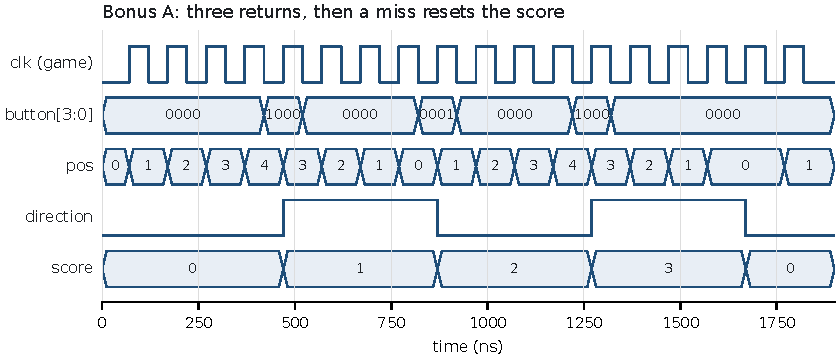
\includegraphics[width=0.92\linewidth]{figures/lab06_pingpong_wave.pdf}
\caption{Bonus A: \sig{pos} bounces 0$\to$4$\to$0, \sig{direction} flips on each return.}\label{fig:pp}
\end{figure}

\subsection{B -- Ping-pong, single clock domain}
The second version keeps the whole design on the \SI{50}{MHz} clock. A \sig{pulse\_generator} emits a
one-cycle \sig{tick} every $\text{max\_count}+1$ cycles (\SI{0.2}{s} at level 0, halving per level) and the
game logic only moves the light when \sig{tick} is high -- a clock \emph{enable} instead of a derived clock.
Button edges are detected in the fast domain, so even a short press is registered. Reaching level 9 wins
(all LEDs on). The testbench plays nine correct returns and reaches the win state, and measures the
level-9 tick period: \num{20001} cycles, as designed.

\subsection{Observations}
\begin{itemize}
  \item Doubling the speed per level quickly exceeds human reaction time ($\approx$\SI{0.2}{s}): in
        version A a step is shorter than \SI{0.2}{s} from level 4, in version B from level 1. A gentler
        progression (e.g.\ $\times1.25$ per level) would make the later levels playable.
  \item In version B a miss is not penalised and repeated presses during one visit to an end each add a
        level. Counting at most one return per visit (and resetting on a miss, as in version A) would
        restore the intended rules.
  \item The push buttons are not debounced; a bouncing contact can register several edges. A small
        debounce counter or sampling on the slow tick would avoid this.
\end{itemize}

\section{Implementation results}
\begin{table}[h]
\centering\small
\caption{Vivado post-implementation results (XC7Z010).}
\begin{tabular}{@{}lrrrr@{}}
\toprule
Design & LUTs & Flip-flops & WNS (ns) & Timing\\
\midrule
Part 2 -- LED flow & 39 & 70 & 15.461 & met\\
Part 3 -- reaction game (block design) & 28 & 32 & 16.215 & met\\
Part 4 -- LED flow clocked by the PS & 40 & 70 & 15.246 & met\\
Bonus A -- ping-pong (block design) & 49 & 44 & 15.189 & met\\
Bonus B -- ping-pong, single clock & 78 & 48 & 13.266 & met\\
\bottomrule
\end{tabular}
\end{table}

\section{Verification summary}
\begin{table}[h]
\centering\small
\begin{tabularx}{\linewidth}{@{}lXr@{}}
\toprule
Testbench & What is checked & Result\\
\midrule
\sig{tb\_clk\_led} & LED equals the clock & \pass\\
\sig{tb\_led\_blink} & 25 toggles, each after exactly one half-period & \pass\\
\sig{tb\_led\_flow} (Parts 2, 4) & 20 steps of the pattern; step time after the speed buttons & \pass\\
\sig{tb\_mini\_game} & four hits $\to$ win; hit + miss $\to$ level 0 & \pass\\
\sig{tb\_ping\_pong} & three returns $\to$ score 3; miss $\to$ score 0 & \pass\\
\sig{tb\_ping\_pong\_v2} & nine returns $\to$ win; tick period at level 9 & \pass\\
\bottomrule
\end{tabularx}
\end{table}
The cleaned code contains no functional changes for this experiment; the block designs are provided as
equivalent RTL top levels (\sig{reaction\_game\_top}, \sig{ping\_pong\_top}) together with the original
\texttt{.bd} files.

\section{Conclusion}
A clock divider turns the \SI{50}{MHz} oscillator into human-scale timing, and registers that change the
divider at run time give speed control and level-dependent games. The block-design projects show how RTL
modules are combined in IP Integrator, including feedback from the game logic to its own clock and, in
Part 4, a PL clock supplied by the ARM processing system. The second ping-pong design illustrates the
preferred style for FPGA logic: one clock domain with enable pulses.

\end{document}
